\section{Adverb}

\begin{table}[h]
	\caption{Adverb characteristics}
	\begin{tabular}{ll}
		\textbf{Title}              & \textbf{Value}      \\
		Semantic value              & Attribute           \\
		Category                    & Independent         \\
		Subcategory                 & Nominal             \\
		Alteration                  & Comparison          \\
		Alteration parameters       & Degree              \\
		Differentiation parameters  & Type, Group
	\end{tabular}
\end{table}

There are different words that cannot be alternated. The biggest class of such words is adverb. It unites a number of groups adverbs can be divided into.

First of all, you should know that adverbs\index{adverb} can be divided into three types, depending on the form they have: \textit{primary} (P), \textit{secondary} (S) and \textit{derivative} (D). When we speak about adverb groups, these letters will be written next to the adverb to help you easier differentiate these types.

\underline{Primary\index{adverb!primary}} adverbs have been formed long ago and we study it as a whole word, without an easy-found root.

\textbf{Examples:}

\textit{Nyne} - Now

\textit{Dy} - When

\textit{De} - Where

\underline{Secondary\index{adverb!secondary}} adverbs have been formed from two words (or a phrase) or from a frozen word form. 

\textbf{Examples:}

\textit{Vdomu} - At home

\textit{Nazad} - Backwards

\underline{Derivative\index{adverb!derivative}} adverbs have been shifted semantically from an adjective. It is the most common type of adverbs. This form usually corresponds with -LY adverbs in English.

\textbf{Examples:}

\textit{Hlådno} - Cold, Coldly

\textit{Věčno} - Eternally

Now let us talk about groups of adverbs. One distinguishes two main types of adverbs: \textit{Significant} and \textit{Demonstrative} \cite{belorussian}. Significant adverbs names concrete property or process attributes, while demonstrative adverbs only refer to these attributes or have an indication of the common nature.

\begin{figure}
	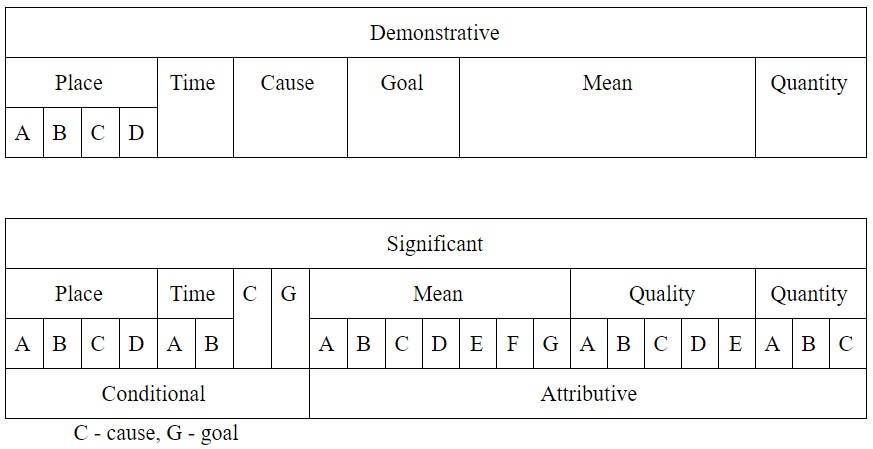
\includegraphics[width=\linewidth]{./sources/adverbs.jpg}
	\caption{Categories of adverbs}
	\label{fig:adverbs}
\end{figure}

\subsection{Demonstrative adverbs}

There are six categories of demonstrative\index{adverb!demonstrative} adverbs. They are adverbs of place, time. cause. goal, mean, quantity.

1. \textbf{Demonstrative adverbs of place.}

Let’s speak about subcategories of this adverbs. 

A. \textit{Adverbs indicating the place of action.}

Question: \textit{Where? (Kųde?)}

Here - \textit{Tut, zdě}

There - \textit{Tamo, tųde}

Everywhere - \textit{Vsëde, vsüdu, vsëkųde}

Nowhere - \textit{Nide, nikųde}

Somewhere - \textit{Něde, někųde}

B. \textit{Adverbs indicating the place where action is directed. }

Question: \textit{Whither? (Kųda?)}

Here - \textit{Nazdě, süda}

There - \textit{Tųda, natųde, natamo}

Everywhere - \textit{Navsękųde, vsękųda}

Nowhere - \textit{Nanikųde, nikųda}

Somewhere - \textit{Naněkųde, někųda}


C. \textit{Adverbs indicating the place of action’s start.}

Question: \textit{Whence? (Odkųde?)}

Here - \textit{Odzdě, odsüda}

There - \textit{Odtųda}

Everywhere - \textit{Odvsękųda}

Nowhere - \textit{Odnikųda}

Somewhere - \textit{Odněkųda}


D. \textit{Adverbs indicating the place of action’s end.}

Question: \textit{Where? How far? (Dokųde?)}

(Up to) here - \textit{Dozdě}

There - \textit{Dotųde, dotamo}

Everywhere - \textit{Dovsękųde}

Nowhere - \textit{Donikųde}

Somewhere - \textit{Doněkųde}


2. \textbf{Demonstrative adverbs of time}

Question: \textit{When? (Koĝda?)}

Now - \textit{Nyně, sëdy}

Afterwards - \textit{Poslě, potym}

Later - \textit{Pozdě, po-pozdno}
%TODO: Pozdne??%

Then - \textit{Poslě, potym}

Once - \textit{Jednađy}

Sometimes - \textit{Něĝda, nědy}

Ever - \textit{Něĝda, nědy}

Never - \textit{Niĝda, nidy}

Always - \textit{Vsëĝda, vsëdy}

3. \textbf{Demonstrative adverbs of cause}

Question: \textit{Why? (Čomu?)}

Therefore - \textit{Slědno}

Because - \textit{Bo, tomu če}

Thus - \textit{Tako}

Somehow - \textit{Nějako}

4. \textbf{Demonstrative adverbs of goal}

Question: \textit{For what? (Za čto?)}

For - \textit{Za da, dlä}

In order to - \textit{Dlä}

So as to - \textit{Za da}

5. \textbf{Demonstrative adverbs of mean}

Question: \textit{How? (Kako?)}

So - \textit{Tako}

Likewise - \textit{Podobno}

Somehow - \textit{Nějako}

Otherwise - \textit{Drugo}

Nohow - \textit{Nijako}

Like that - \textit{Kakto (Kako to)}

That way - \textit{Tako}

Anyhow - \textit{Nějako}

Differently - \textit{Ïno}

6.\textbf{ Demonstrative adverbs of quantity}

Question: \textit{How much? (Kolïko?)}

So much - \textit{Tako mnogo}

Few - \textit{Několïko}

Some - \textit{Několïko}

Several - \textit{Několïko}

Nary - \textit{Malo}


\subsection{Significant adverbs}

Significant\index{adverb!significant} adverbs are often divided into two large subcategories - conditional and attributive adverbs. \textit{Conditional} adverbs shows the conditions of the action took place - place, time, cause, goal. \textit{Attributive} shows the attributes of the action - the mean of the action. its quality and its quantity.

1. \textbf{Significant adverbs of place.}

A. \textit{Adverbs indicating the place of action.}

Question: \textit{Where? (Kųde?)}

Next to (close to) - \textit{Blïzko do}

Ahead - \textit{Upredï}

Opposite - \textit{Naprotï}

Around - \textit{Okolo}

Far - \textit{Dalïko}

Not far - \textit{Nedalïko}

Among - \textit{Među, sredï}

Between - \textit{Među}

At home -\textit{ Doma, vdomu}

Upstairs - \textit{Uvòrhu, vòrhu}

Downstairs - \textit{Unïzu, nïzu}

B. \textit{Adverbs indicating the place where action is directed. }

Question:\textit{ Whither? (Kųda?)}

Ahead - \textit{Upred}

To the right - \textit{Uděsno}

Upwards - \textit{Uvòrh}

Sideways - \textit{Uboku}

Downwards - \textit{Unïz}

Opposite - \textit{Naprotiv}

Home - \textit{Dodomu}

C. \textit{Adverbs indicating the place of action’s start.}

Question: \textit{Whence? (Odkųde?)}

From upstairs - \textit{Zvòrhu}

From downstairs - \textit{Znïzu}

From the right - \textit{Zděsnu}

From the left - \textit{Zlěvu}

D. \textit{Adverbs indicating the place of action’s end.}

Question: \textit{Where? How far? (Dokųde?)}

Up to the top - \textit{Dovòrha}

Down to the bottom - \textit{Donïza}

2. \textbf{Significant adverbs of time}

Question: \textit{When? (Koĝda?)}

\textit{A. With relative time value}

Now - \textit{Nyně}

Already - \textit{Juž}

Soon - \textit{Skoro}

Always - \textit{Vsëĝda}

Long ago - \textit{Davno}

Recently - \textit{Nedavno}

Earlier - \textit{Ráno}

\textit{B. With the value of while when the action is executed.}

Today - \textit{Dnësj}

Yesterday - \textit{Včera}

The day before yesterday - \textit{Zadvčera}

In the afternoon - \textit{Dnëm}

In the night - \textit{Nočïü}

In the morning - \textit{Jutrom}

Before the dawn - \textit{Predutrom}

In the evening - \textit{Večorom}

In spring - \textit{Věsnoju}

In autumn - \textit{Jesenïü}

In winter - \textit{Zimoju}

In summer - \textit{Lětom}

3. \textbf{Significant adverbs of cause}

Question: \textit{Why? (Čomu?)}

Accidentally - \textit{Slučaǐno}

Intentionally - \textit{Umysëlno}

4. \textbf{Significant adverbs of goal}

Question: For what? (Za čto?)

Cattily - \textit{Nazlo}

For memory - \textit{Napamętj}

Further let’s speak about attributive adverbs.

1. \textbf{Significant adverbs of mean}

Question: \textit{How? (Kako?)}

\textit{A. With value of forming an aciton}

Again - \textit{Znovu}

Firstly - \textit{Pòrvo}

Gradually - \textit{Postepno}

Immediately - \textit{Zrazu}

\textit{B. With value of executing the action}

Sometimes - \textit{Něĝda}

Annually - \textit{Vsękoročno}

Continuously - \textit{Bezostanno}

\textit{C. With value of action subject state}

Grungingly - \textit{Nehòtno}

Seriously - \textit{Považno}

Silently - \textit{Mòlčno}

\textit{D. With value of action result}

For long - \textit{Nadôlgo}

Past - \textit{Mïmo}

\textit{E. With value of the mean of execution}

Afoot - \textit{Pěhom}

Running - \textit{Běgom}

Aloud - \textit{Naglås, glåsno}

\textit{F. With value of similarity}

Fraternally - \textit{Po-bratóvu}

Our way - \textit{Po našomu}

\textit{G. With value of connection between subjects}

Together - \textit{Zajedno}

Jointly - \textit{Splåtno}

2. \textbf{Significant adverbs of quality}

Question: \textit{How? (Kako?)}

\textit{A. With value of color}


\textit{B. With value of length}

\textit{C. With value of action/state expressing measure}

\textit{D. With value of action/state expressing estimation}

\textit{E. With value of state}

3.\textbf{ Significant adverbs of quantity}

Question: \textit{How much? (Kolïko?)}

\textit{A. With value of intensity}

Very - \textit{Vëlïmi}

Almost - \textit{Blïzko}

A bit - \textit{Malko}

\textit{B. With value of measure}

Many - \textit{Mnogo}

Little - \textit{Malo}

More - \textit{Ješto}

\textit{C. With value of growth limit}

Forever - \textit{Navsëdy}

To the end - \textit{Dokonca}

Too long - \textit{Predôlgo}

\subsection{Degrees of comparison}

Likewise adjectives, adverbs have three degrees of comparison\index{comparison}. Moreover, there are synthetic and analytic forms too. 

Remember (look at paragraph about adjective degrees of comparison), that there are three degrees: positive, comparative and superlative.

\textbf{Synthetic forms}

Comparative\index{comparison!synthetic} form is made by adding to the word base the suffix “ěǐ’. Unlike adjectives, this is the only suffix to create a comparative form (compare with suffixes “ëǐ”, “aǐ” for hard and soft bases in adjectives). 

\underline{Examples:}

\textit{Mnogo - Množěǐ}

\textit{Sïnë - Sïněǐ}

Superlative form is made so as it is in adjectives - adding a prefix “naǐ-” to the comparative form.

\textbf{Analytic forms}

Analytic\index{comparison!analytic} forms provide simple ways of creating comparative and superlative forms without modifying the word itself. There are two types of adverb analytic comparison.

\textbf{Using prefixes}

Comparative form is created by adding prefix “po-” through a defis ro a positive form. Superlative form is created by adding prefix “naǐ-” through a defis to the positive form.

\underline{Examples:}

\textit{Mnogo - po-mnogo - naǐ-mnogo}

\textbf{Using an auxiliary adverb}

To the positive form you should add an auxiliary adverb in comparative or superlative form.

\begin{table}[!htb]
	\caption{Auxiliary adverb for analytic comparison}
	\begin{tabular}{lll}
		Auxiliary adverb
		& Comparative form
		& Superlative form \\
		more & bolěǐ & naǐbolěǐ \\
		less & mëněǐ & naǐmëněǐ \\
	\end{tabular}
\end{table}

\underline{Examples:}

\textit{Mnogo - bolěǐ mnogo - naǐbolěǐ mnogo}

You can use both synthetic and analytic forms at the same time.
